%; whizzy document
% latex beamer presentation.
% platex, latex-beamer でコンパイルすることを想定。 

%     Tokyo Debian Meeting resources
%     Copyright (C) 2006 Junichi Uekawa

%     This program is free software; you can redistribute it and/or modify
%     it under the terms of the GNU General Public License as published by
%     the Free Software Foundation; either version 2 of the License, or
%     (at your option) any later version.

%     This program is distributed in the hope that it will be useful,
%     but WITHOUT ANY WARRANTY; without even the implied warranty of
%     MERCHANTABILITY or FITNESS FOR A PARTICULAR PURPOSE.  See the
%     GNU General Public License for more details.

%     You should have received a copy of the GNU General Public License
%     along with this program; if not, write to the Free Software
%     Foundation, Inc., 51 Franklin St, Fifth Floor, Boston, MA  02110-1301 USA

% 実行順番
% sudo  ~/bin/usb-macbook-ir.c &
% real presentation (shell-command (concat "DISPLAY=:0.1 xpdf -fullscreen " (replace-regexp-in-string "tex$" "pdf"(buffer-file-name)) "&"))
% DISPLAY=:0.1 xpdf -fullscreen 

\documentclass[cjk,dvipdfmx]{beamer}
\usetheme{Warsaw}
%  preview (shell-command (concat "xpdf " (replace-regexp-in-string "tex$" "pdf"(buffer-file-name)) "&"))
%  presentation (shell-command (concat "xpdf -fullscreen " (replace-regexp-in-string "tex$" "pdf"(buffer-file-name)) "&"))

%http://www.naney.org/diki/dk/hyperref.html
%日本語EUC系環境の時
\AtBeginDvi{\special{pdf:tounicode EUC-UCS2}}
%シフトJIS系環境の時
%\AtBeginDvi{\special{pdf:tounicode 90ms-RKSJ-UCS2}}

\title{東京エリア Debian 勉強会}
\subtitle{資料}
\author{上川 純一 dancer@debian.org\\IRC nick: dancerj}
\date{2006年12月16日}
\logo{
\includegraphics[width=8cm]{image200607/openlogo-light.eps}}

% 三択問題用
\newcounter{santakucounter}
\newcommand{\santaku}[5]{%
\addtocounter{santakucounter}{1}
\frame{\frametitle{問題\arabic{santakucounter}. #1}
%問題\arabic{santakucounter}. #1
\begin{minipage}[t]{0.7\hsize}
 \begin{itemize}
 \item  A #2\\
 \item  B #3\\
 \item  C #4\\
 \end{itemize}
\end{minipage}
}
\frame{\frametitle{問題\arabic{santakucounter}. #1}
%問題\arabic{santakucounter}. #1
\begin{minipage}[t]{0.7\hsize}
\begin{itemize}
\item  A #2\\
\item  B #3\\
\item  C #4\\
\end{itemize}
\end{minipage}
\begin{minipage}[t]{0.2\hsize}
答えは:

\vspace{1cm}

{\huge \hspace{1cm}#5}
\end{minipage}}
}


\begin{document}
\frame{\titlepage{}}

\section{Intro}

\begin{frame}
 \frametitle{本日のagenda}
\begin{minipage}[t]{0.4\hsize}
  \begin{itemize}
  \item 注意事項
	\begin{itemize}
	 \item 飲食禁止
	 \item 政治/宗教/営利活動禁止
	\end{itemize}
  \item 最近事情
  \item 事前課題紹介
  \item quiz
 \end{itemize}
\end{minipage} 
\begin{minipage}[t]{0.4\hsize}
 \begin{itemize}
  \item Bug Squashing Partyについて
  \item 来年の Debian 勉強会を設計する
 \end{itemize}
\end{minipage}
\end{frame}

\section{最近のDebian関連のミーティング報告}

\begin{frame}{最近のDebian関連ミーティング報告}
 \begin{itemize}
  \item Debian勉強会
  \item 関西オープンソース
 \end{itemize}
\end{frame}



\begin{frame}
 \frametitle{10月のDebian勉強会のagenda}
\begin{minipage}[t]{0.4\hsize}
  \begin{itemize}
  \item 注意事項
	\begin{itemize}
	 \item 飲食禁止
	 \item 政治/宗教/営利活動禁止
	\end{itemize}
  \item 最近事情
  \item 事前課題紹介
  \item quiz
 \end{itemize}
\end{minipage} 
\begin{minipage}[t]{0.4\hsize}
\begin{itemize}
  \item スペイン参加報告
  \item flash ねた
  \item apt チューニングねた
 \end{itemize}
\end{minipage}
\end{frame}


\begin{frame}
 \frametitle{KOF Debian BOF のアジェンダ}
\begin{minipage}[t]{0.4\hsize}
  \begin{itemize}
  \item 講師
	\begin{itemize} 
	 \item 上川\\
	       Debian JP 会長
	 \item 岩松\\
	       Debian JP 副会長
	 \item やまね\\
	       po-debconf翻訳職人
	\end{itemize}
 \end{itemize}
\end{minipage} 
\begin{minipage}[t]{0.4\hsize}
 \begin{itemize}
  \item Debian 紹介
  \item Debian JP 紹介
  \item エッチについて
  \item Debconf in Japan 進捗報告
 \end{itemize}
\end{minipage}
\end{frame}

\begin{frame}
 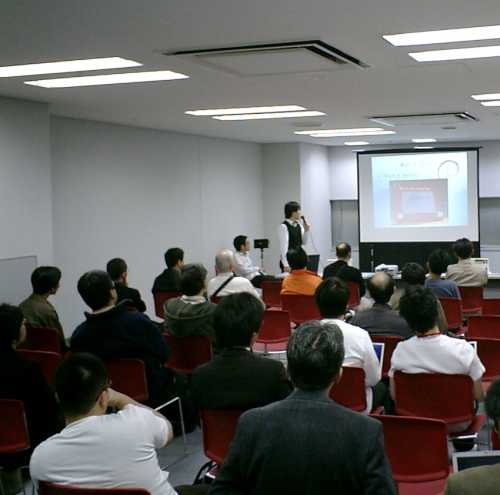
\includegraphics[width=0.8\hsize]{image200611/meeting.jpg}
\end{frame}


\begin{frame}
 \frametitle{関西開催勉強会アジェンダ}
\begin{minipage}[t]{0.35\hsize}
  \begin{itemize}
   \item 今日の講師
   \item 上川\\
	 Debian JP 会長
   \item 岩松\\
	 Debian JP 副会長
 \end{itemize}
\end{minipage} 
\begin{minipage}[t]{0.6\hsize}
 \begin{itemize}
  \item 14:00-14:20 最近の Debian 勉強会の紹介
  \item 14:20-15:00 事前課題紹介
  \item 15:00-15:10 sid を日常環境として使うための注意, 上川
  \item 15:10-15:20 bugreport 論, 上川
  \item 15:30-16:00 パッケージングについて, 岩松
  \item 16:00-16:40 質問コーナー, 各位
  \item 17:00-18:00 京橋に移動
  \item 18:00-20:00 宴会
 \end{itemize}
\end{minipage}
\end{frame}

\begin{frame}
 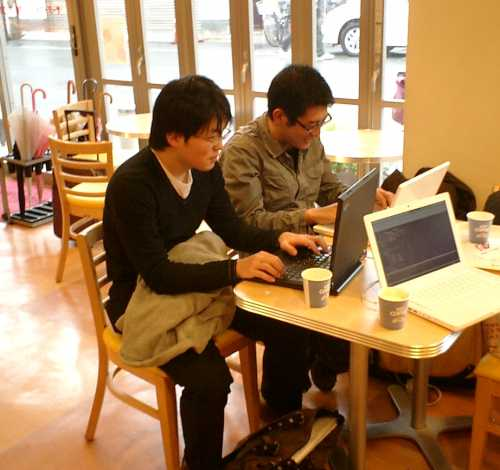
\includegraphics[width=0.8\hsize]{image200611/hack.jpg}
\end{frame}

\begin{frame}
 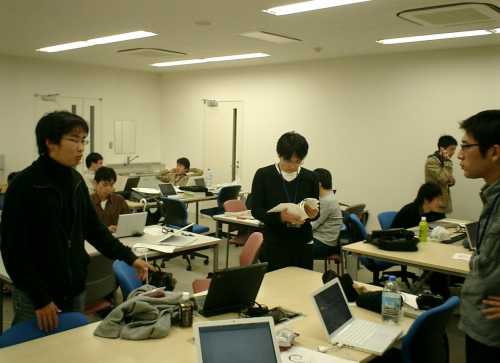
\includegraphics[width=0.8\hsize]{image200612/kansai.jpg}
\end{frame}


\section{事前課題の声}
\begin{frame}

 今回の事前課題は
 「来年のDebian勉強会でやりたいこと」もしくは「来年の
 Debian勉強会のスタイルを提案する」
 というタイトルで200-800文字程度の文章を書いてください。というものでした。
 その課題に対して下記の内容を提出いただきました。
\end{frame}

\begin{frame}
 
 \frametitle{小林儀匡さん}

 『来年のDebian勉強会のスタイルを提案する』

 Debian勉強会もついに2歳を迎え、パッケージ作成作業に関連する各種ツールの
 使い方・Debian Policy Manualの内容・翻訳作業などといった、開発者への入口
 となる情報を提供するテーマは一通り扱ったと思います。それらの内容に大きな
 変化があったらそれは更新する必要がありますし、まだ触れられていないツール
 についても扱う必要があると思いますが、開発者への入口をまとめたドキュメン
 トの提供という当初の大きな目的の一つは大方達成されたのではないでしょうか。
\end{frame}
\begin{frame}
 
 このような状況を鑑みると、これからは、「現在のDebian GNU/Linuxシステムに
 存在する問題点を何かしら見つけて、それについてグループディスカッションの
 ようなかたちで掘り下げ、今後の開発作業に繋げてみる」という問題発見型の勉
 強会も必要になるのではないかと思います。これまでも飲み会で「あれはどうに
 かならないか」と議論になったり、ネットワークの設定についての課題への回答
 を巡って議論になったりしましたが、このような議論をきちんとしたかたちでやっ
 てみる、ということです。理想的には (かなり大きな理想ですが)、本勉強会で
 議論したことをDebian本家のメーリングリストに英語で流して、それを元に何か
 を生み出せればとても素敵だと思います。\end{frame}

\begin{frame}

もちろん、これを毎月行うのはやや負
 担が大きく、実際の作業がなかなか進まないままネタ切れというのがオチになる
 可能性もあるので、これまでのように、会議の報告や「Debianでこんなことをし
 てみた」というネタ的な話、開発関連ツールではないがまとめておくと有用な事
 項 (glibc・Flash・マルチメディア関連・……) のまとめなども混ぜていく必要
 があるかと思いますが……。

  ネタがなくなって勉強会自体がマンネリ化しだらだら続くことのないよう、自分
 ももう少し提供できるネタがないか考え、そして実際に提供しながら臨みたいと
 思う2006年冬です。
\end{frame}

\begin{frame}
 
 \frametitle{前田さん}


 お題「来年のDebian勉強会のスタイルを提案する」として、ワークショップ形式
 で議論するのが良いですね。他の参加者の方と(宴会以外で)話す機会も増えま
 すので。って、今回はもろにそういう形式のようですね。失礼しました。

 あとは、ハンズオンとか。帰宅後に資料を見てやるのも良いのですが、宴会の後、
 帰宅したら寝てしまうので、やはりその場で手を動かす方がより効果が高いかと。
 (次の日だと忘れるか、覚えていてもやらない、という事もままあるので…)
\end{frame}
\begin{frame}
 
 \frametitle{澤田さん}

 スタイルの提案で書きます。「/etc/network/interfacesをさらしてください」
 という事前課題はいろいろバッドノウハウが出て盛り上がったことと思われます
 (諸事情により参加しませんでしたが)。

 そこで今後も、ある事項について、「私はこうやっています」という事前課題を
 書いてもらい、バッドノウハウとしてまとめるというのはどうでしょうか?例え
 ば、「apt-get upgradeしたらパッケージが壊れていてアップグレードが完了し
 ない。怒りのBTSは当然投げるとして、とりあえずどう対処する?」とか、「バッ
 クアップ、何使ってますか?何バックアップしてますか?」(「バックアップ 
 Debian」でググるとやまねさんの過去の投稿がありますね)とか、知っている人
 は知っているというバッドノウハウが多いと思います。
\end{frame}
\begin{frame}
 

 \frametitle{小室 文さん}

 「来年のDebian勉強会でやりたいこと」
 勉強会でやりたい事ではないですが、女の子の参加者がもっと増えるように地道
 な活動?をしようと決めてます。いないはずはないので、勉強会に来てもらえる
 ようにいろんな所で探したいと思います。


 「来年のDebian勉強会のスタイルを提案する」
 継続して多くの人が参加しないのは、参加者のレベルに(しょうがない事ですが)
 バラツキがある為だと思います。ちょっと分からない単語や内容を後で調べてみ
 よう、というレベルの開きではなくて、何の事かすら分からない事が時々ありま
 す(特にカーネル関係は難しい…)。debian勉強会+初級・中級者向け勉強会が
 あったら、利用者も増えて階段を上る感じでいいかもしれません。
 (有志なので難しいとは思いますが。。。)
\end{frame}
\begin{frame}
 
 \frametitle{キタハラさん}

    現在のDebian勉強会のスタイルに不満点は無いので
 すが・・・

    最近、初心者向けの某勉強会で輪読していて、20
 ン年前の学生時代の雰囲気を堪能して来ました。

    輪読は、対象となる資料を「事前に読んで」おき、
 その時に理解できなかった所や疑問に思った所を、当日
 「有識者と共に」ディスカッションする事により、「他
 の参加者の視点」と共に対象の事柄を「より深く理解」
 できるという利点があると思います。

    現在のDebian勉強会で輪読を行うのは、少々無理が
 あるかもしれませんが(別枠で初心者向け『徹底入門
 第4版 〜etch対応(仮?)』の輪読(読書会)があった
 ら参加したいなぁ〜)、適当な長さの資料を事前に読ん
 でおき、当日参加者が順番に読んで、疑問点や注意点を
 話し合うコーナーを作るという形ならば、実現可能かも
 しれません。
\end{frame}
\begin{frame}
 
 \frametitle{青木さん}

 「来年のDebian勉強会でやりたいこと」というお題をいただきましたので
 おひとつ話させていただきます。

 今までDebian勉強会に関して開催形態(課題があること)に減らず口を叩いた
 以外出席すらしてきていない私がDebian勉強会で何をするかを語るのもチョッと
 変な気がします。

 でもソフト関係で食ってるわけでもないわたしが今までDEBIANでいろいろしてきた
 経験を、長く終わりの見えないNMプロセスに取り組もうとされている方々と共有す
 る機会がもてればいいのではないかと考えています。

 それにDEBIANは英語でのコミュニケーションがDDとして続く必須条件という状況
 もあります。これって多くの日本人にとって結構気の重いものでは無いでしょうか?
\end{frame}

\begin{frame}
 
 これらの障害のあるDEBIANですが、だからこそ日本人が参加し、日本語環境を世界
 中どこにいても誰でも使えるようにしようではありませんか?いま日本語環境をサ
 ポートしているひとは少ないので、是非協力してくれるひとを見付けたいものです。

 それから、内容が古くなったのが否めないDEBIAN REFERENCEをもう少しバージョン
 アップに影響されないようにしたかたちにする、そしてXMLに変更する作業をどな
 たか見付けられないかなという勝手な期待もあります。
\end{frame}


\begin{frame}
 
 \frametitle{上川}

 勉強会のスタイルは、理由があってこうなっている部分もありますが、最初にこ
 うしたからこうなっている、ということで特に理由があって決まっていない部分
 もあります。たまにはそういう部分に変化を加えていかないと、マンネリになっ
 てしまい、飽きてくるので、変化させることは重要だと思っています。是非みな
 さまのアイデアを活用して何か違う形を採り入れたいとおもっております。
\end{frame}


\section{DWNQuiz}
%% debianmeetingresume200612.texから以下コピー
\subsection{2006年41号}
\url{http://www.debian.org/News/weekly/2006/41/}
にある11月28日版です。

\santaku
{Debian Conference 7 日程が決まりました。いつからでしょうか。}
{4/1}
{5/22}
{6/17}
{C}


\santaku
{Debian Project に新しい開発用マシンが導入されました。どのマシンでしょうか。}
{Sun Fire T2000}
{Sony Playstation 3}
{TiVo Series2 DVR}
{A}


\subsection{Debian 勉強会の一年をしめくくる}

\begin{frame}{Debian JPとDebian 勉強会}
個人的な理想

\includegraphics[width=0.7\hsize]{image200610/debianstructure.eps}
\end{frame}

\begin{frame}

\begin{minipage}{0.6\hsize}
 \includegraphics[width=0.5\hsize]{image200612/hierarchy.eps}
\end{minipage}
\begin{minipage}{0.6\hsize}
 \begin{itemize}
  \item Debian 勉強会では、Power Users から NM / DD への道を
 \end{itemize}
\end{minipage}
\end{frame}


\begin{frame}{新規の参加者}

\begin{itemize}
 \item 2005年1月: 20 人
 \item 2005年2月: 6 人
 \item 2005年のこり: 12 人
 \item 2006年 -6月: 9人
 \item 2006年 -10月: 14人
\end{itemize}

\end{frame}

\begin{frame}{新規に参加して二度以上参加してくれた参加者の数}
 
\begin{itemize}
 \item 2005年: 39人中 21人
 \item 2006年上半期 (-6月): 9人中 5人
 \item 2006年下半期 (-10月): 14人中 2人
\end{itemize}

\end{frame}


\begin{frame}{Debian Developer比率}

 \begin{itemize}
 \item 2005年:39人中 DD 4 人? NM 3 人
 \item 2006年 -10月:36人中 DD 6 人 NM 6 人
 \end{itemize}
\end{frame}

\begin{frame}{参加人数}
 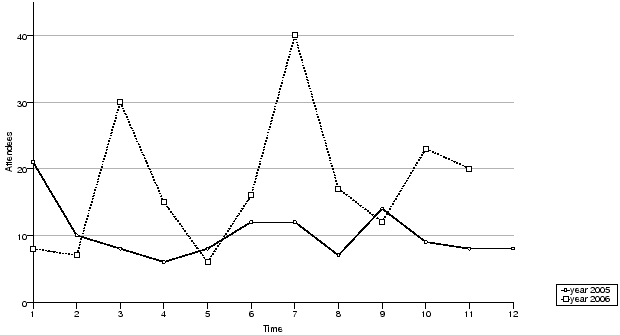
\includegraphics[width=1\hsize]{image200612/people-chart.png}
\end{frame}

\begin{frame}{2005年}
  \begin{tabular}{|l|c|}
 \hline
   & 参加人数 \\
 \hline
   2005年1月 & 21 \\
   2005年2月 & 10 \\
   2005年3月 & 8\\
   2005年4月 & 6\\
   2005年5月 & 8\\
   2005年6月 & 12\\
   2005年7月 & 12\\
   2005年8月 & 7\\
   2005年9月 & 14\\
   2005年10月 & 9\\
   2005年11月 & 8\\
   2005年12月 & 8 \\
 \hline
  \end{tabular}
\end{frame}

\begin{frame}{2006年}
   \begin{tabular}{|l|c|l|}
 \hline
 & 参加人数 & \\
 \hline
 2006年1月 & 8 & policy,Debian勉強会でやりたいこと\\
 2006年2月 & 7 & policy, multimedia \\
 2006年3月 & 30 & OSC: debian勉強会,sid \\
 2006年4月 & 15 & policy, latex \\
 2006年5月 & 6 & mexico \\
 2006年6月 & 16 & debconf, cowdancer\\
 2006年7月 & 40 & OSC-Do: MacBook Debian \\
 2006年8月 & 17 & 13執念 \\
 2006年9月 & 12 & 翻訳、Debian-specific、oprofile \\
 2006年10月 & 23 & network, i18n会議、Flash、apt \\
 2006年11月 & 20 & 関西: bug, sid, packaging \\
 2006年12月 & 14 & 忘年会 \\
 \hline
  \end{tabular}
\end{frame}

\begin{frame}
じゃあ来年どうしようか? 
\end{frame}

\subsection{今後のイベント}

\begin{frame}
 \frametitle{今後のイベント}
 \begin{itemize}
  \item Debian 勉強会開催
  \item Debian Conference 2007 Edinburgh 2007年6月
  \item Debian 14周年 2007年8月16日
  \item Debian 15周年 2008年8月16日
 \end{itemize}
\end{frame}

\subsection{今後のイベント}

\begin{frame}
 \frametitle{宴会会場}
 \begin{itemize}
  \item 会場:荻窪 卯(うさぎ)
  \item 時間:21:30-
  \item 集合場所: この建物 1F のところ
  \item 注意事項
	\begin{itemize}
	 \item 終電の時間をちゃんとしらべていきましょう
	\end{itemize}
 \end{itemize}
\end{frame}


\section{wrap-up}
\begin{frame}
 \frametitle{今日のまとめ}
 \begin{itemize}
  \item まとめ
 \end{itemize}
\end{frame}

\end{document}
